\documentclass[aspectratio=169,11pt]{beamer}

\usetheme{Madrid}
\usecolortheme{seahorse}
\setbeamertemplate{navigation symbols}{}
\setbeamertemplate{caption}[numbered]

\usepackage[utf8]{inputenc}
\usepackage[T1]{fontenc}
\usepackage{lmodern}
\usepackage[brazil]{babel}
\usepackage{graphicx}
\usepackage{booktabs}
\usepackage{array}
\usepackage{tikz}
\usepackage{xcolor}
\usepackage{seqsplit}
\usepackage{microtype}

\usetikzlibrary{arrows.meta, positioning, shapes.geometric, fit, calc}

\definecolor{genesysBlue}{RGB}{30,72,130}
\definecolor{genesysGreen}{RGB}{42,125,92}
\definecolor{genesysOrange}{RGB}{206,120,45}
\definecolor{softBlue}{RGB}{232,240,252}
\definecolor{softGreen}{RGB}{232,248,239}
\definecolor{softOrange}{RGB}{255,243,226}
\definecolor{softRed}{RGB}{252,232,232}
\definecolor{darkText}{RGB}{30,38,48}

\setbeamercolor{title}{fg=white,bg=genesysBlue}
\setbeamercolor{frametitle}{fg=white,bg=genesysBlue}
\setbeamercolor{structure}{fg=genesysBlue}
\setbeamercolor{block title}{fg=white,bg=genesysBlue}
\setbeamercolor{block body}{fg=darkText,bg=softBlue}
\setbeamercolor{alerted text}{fg=genesysOrange}

\newcommand{\codeid}[1]{\texttt{\detokenize{#1}}}
\newcommand{\smallcode}[1]{{\scriptsize\texttt{\detokenize{#1}}}}

\tikzset{
    classbox/.style={
        rectangle,
        draw=genesysBlue!70,
        rounded corners=2pt,
        align=left,
        fill=softBlue,
        minimum width=2.15cm,
        minimum height=0.72cm,
        font=\tiny
    },
    compbox/.style={
        rectangle,
        draw=genesysGreen!75,
        rounded corners=2pt,
        align=center,
        fill=softGreen,
        minimum width=2.15cm,
        minimum height=0.75cm,
        font=\tiny
    },
    statebox/.style={
        rectangle,
        draw=genesysOrange!80,
        rounded corners=2pt,
        align=center,
        fill=softOrange,
        minimum width=2.2cm,
        minimum height=0.72cm,
        font=\tiny
    },
    failbox/.style={
        rectangle,
        draw=red!65,
        rounded corners=2pt,
        align=center,
        fill=softRed,
        minimum width=2.2cm,
        minimum height=0.72cm,
        font=\tiny
    },
    flowarrow/.style={-{Latex[length=2mm]}, thick, draw=darkText!75},
    faintarrow/.style={-{Latex[length=1.8mm]}, thick, draw=darkText!45},
    lifeline/.style={draw, dashed, gray!65},
    note/.style={rectangle, rounded corners=2pt, fill=yellow!18, draw=yellow!55!black, align=center, font=\tiny}
}

\title[Parser Din\^amico no GenESyS]{Mecanismo de Atualiza\c{c}\~ao Din\^amica do Parser no GenESyS}
\subtitle{Pr\'evia para apresenta\c{c}\~ao em simp\'osio}
\author[Vicente, Ricardo, Eduardo]{
Vicente Cardoso dos Santos \and
Ricardo Henrique Medeiros Pereira \and
Eduardo Bischoff Grasel
}
\institute[UFSC]{Universidade Federal de Santa Catarina \\ INE5425 -- Modelagem e Simula\c{c}\~ao}
\date{}

\begin{document}

\begin{frame}
    \titlepage
\end{frame}

\begin{frame}{Roteiro da Pr\'evia}
    \begin{columns}[T,onlytextwidth]
        \column{0.48\textwidth}
        \begin{block}{1. Apresentando o projeto}
            Problema, objetivo e vis\~ao geral.
        \end{block}
        \begin{block}{2. Desenvolvimento}
            Contratos, lazy reload, gera\c{c}\~ao, compila\c{c}\~ao e runtime.
        \end{block}
        \column{0.48\textwidth}
        \begin{block}{3. Testes}
            Valida\c{c}\~ao do fluxo completo e das falhas.
        \end{block}
        \begin{block}{4. Resultados}
            Demonstra\c{c}\~ao, evid\^encias e impacto.
        \end{block}
    \end{columns}
\end{frame}

\section{Apresentando o Projeto}

\begin{frame}{Problema: Modelo Extens\'ivel, Parser Fixo}
    \begin{columns}[T,onlytextwidth]
        \column{0.48\textwidth}
        \begin{block}{Modelo}
            \begin{itemize}
                \item Recebe plugins.
                \item Ganha novas defini\c{c}\~oes de dados.
                \item Pode incorporar novas fun\c{c}\~oes conceituais.
            \end{itemize}
        \end{block}

        \column{0.48\textwidth}
        \begin{block}{Parser original}
            \begin{itemize}
                \item Depende de Bison/Flex.
                \item Reconhece tokens e regras j\'a compilados.
                \item N\~ao acompanha automaticamente cada plugin.
            \end{itemize}
        \end{block}
    \end{columns}

    \vspace{0.35cm}
    \centering
    \begin{tikzpicture}[node distance=1.0cm]
        \node[compbox, minimum width=3.0cm] (plugin) {Nova extens\~ao};
        \node[statebox, right=2.2cm of plugin, minimum width=3.4cm] (parser) {Parser fixo};
        \node[failbox, right=2.2cm of parser, minimum width=3.2cm] (erro) {Express\~ao n\~ao reconhecida};
        \draw[flowarrow] (plugin) -- node[above, font=\scriptsize]{adiciona conceito} (parser);
        \draw[flowarrow] (parser) -- node[above, font=\scriptsize]{sem regra} (erro);
    \end{tikzpicture}
\end{frame}

\begin{frame}{Objetivo}
    \begin{block}{Objetivo central}
        Permitir que extens\~oes declarem mudan\c{c}as de linguagem e que o GenESyS atualize o parser automaticamente.
    \end{block}

    \vspace{0.2cm}
    \begin{columns}[T,onlytextwidth]
        \column{0.24\textwidth}
        \begin{block}{Declarar}
            Plugin informa tokens, regras e produ\c{c}\~oes.
        \end{block}
        \column{0.24\textwidth}
        \begin{block}{Agregar}
            Kernel coleta contribui\c{c}\~oes do modelo.
        \end{block}
        \column{0.24\textwidth}
        \begin{block}{Gerar}
            Bison/Flex e C++ produzem nova biblioteca.
        \end{block}
        \column{0.24\textwidth}
        \begin{block}{Conectar}
            Runtime troca o parser ativo com seguran\c{c}a.
        \end{block}
    \end{columns}
\end{frame}

\begin{frame}{Vis\~ao Geral da Solu\c{c}\~ao}
    \centering
    \begin{tikzpicture}[node distance=0.9cm and 0.55cm]
        \node[compbox] (ext) {Extens\~ao};
        \node[compbox, right=of ext] (changes) {\codeid{ParserChangesInformation}};
        \node[statebox, right=of changes] (stale) {Marca\\stale};
        \node[statebox, right=of stale] (reload) {\codeid{parseExpression}\\dispara reload};
        \node[compbox, below=0.85cm of reload] (pm) {\codeid{ParserManager}};
        \node[compbox, left=of pm] (tool) {Bison/Flex\\+ C++};
        \node[compbox, left=of tool] (so) {Biblioteca\\\codeid{.so}};
        \node[statebox, left=of so] (newp) {Novo parser\\ativo};

        \draw[flowarrow] (ext) -- (changes);
        \draw[flowarrow] (changes) -- (stale);
        \draw[flowarrow] (stale) -- (reload);
        \draw[flowarrow] (reload) -- (pm);
        \draw[flowarrow] (pm) -- (tool);
        \draw[flowarrow] (tool) -- (so);
        \draw[flowarrow] (so) -- (newp);
    \end{tikzpicture}

    \vspace{0.35cm}
    \begin{block}{Ideia-chave}
        A extens\~ao declara; o kernel gera e conecta; o modelo usa o parser atualizado.
    \end{block}
\end{frame}

\section{Desenvolvimento}

\begin{frame}{Contratos Aproveitados e Completados}
    \begin{columns}[T,onlytextwidth]
        \column{0.48\textwidth}
        \begin{block}{J\'a previsto}
            \begin{itemize}
                \item \codeid{ParserChangesInformation}
                \item \codeid{_getParserChangesInformation()}
                \item \codeid{ParserManager}
                \item Marcadores em Bison/Flex
            \end{itemize}
        \end{block}
        \column{0.48\textwidth}
        \begin{block}{Implementado}
            \begin{itemize}
                \item Campos l\'exicos e \codeid{hasChanges()}
                \item Agrega\c{c}\~ao de mudan\c{c}as
                \item Gera\c{c}\~ao da \codeid{.so}
                \item Conex\~ao via \codeid{dlopen}/\codeid{dlsym}
            \end{itemize}
        \end{block}
    \end{columns}

    \vspace{0.25cm}
    \begin{alertblock}{Decis\~ao}
        Completar a arquitetura existente, preservando os arquivos-base como fonte de verdade.
    \end{alertblock}
\end{frame}

\begin{frame}{Contrato de Mudan\c{c}as}
    \begin{columns}[T,onlytextwidth]
        \column{0.54\textwidth}
        \begin{block}{\codeid{ParserChangesInformation}}
            Pacote de fragmentos que a extens\~ao entrega ao kernel.
        \end{block}

        \begin{itemize}
            \item Includes e tipos sem\^anticos.
            \item Tokens e produ\c{c}\~oes Bison.
            \item Regras e literais Flex.
            \item \codeid{hasChanges()} evita recompila\c{c}\~ao vazia.
        \end{itemize}

        \column{0.42\textwidth}
        \begin{tikzpicture}[node distance=0.55cm]
            \node[compbox, minimum width=3.5cm] (pci) {\codeid{ParserChangesInformation}};
            \node[statebox, below=of pci, minimum width=3.5cm] (bison) {Fragmentos Bison};
            \node[statebox, below=of bison, minimum width=3.5cm] (flex) {Fragmentos Flex};
            \node[statebox, below=of flex, minimum width=3.5cm] (valid) {\codeid{hasChanges()}};
            \draw[flowarrow] (pci) -- (bison);
            \draw[flowarrow] (bison) -- (flex);
            \draw[flowarrow] (flex) -- (valid);
        \end{tikzpicture}
    \end{columns}
\end{frame}

\begin{frame}{Lazy Reload no Ciclo do Modelo}
    \begin{columns}[T,onlytextwidth]
        \column{0.46\textwidth}
        \begin{block}{Na inser\c{c}\~ao}
            \codeid{ModelDataManager::insert()} detecta mudan\c{c}as e marca o parser como stale.
        \end{block}
        \column{0.46\textwidth}
        \begin{block}{No primeiro uso}
            \codeid{Model::parseExpression()} sincroniza a linguagem antes de avaliar.
        \end{block}
    \end{columns}

    \vspace{0.4cm}
    \centering
    \begin{tikzpicture}[node distance=0.85cm]
        \node[compbox, minimum width=2.8cm] (insert) {Inserir extens\~ao};
        \node[statebox, right=of insert, minimum width=2.8cm] (stale) {Parser stale};
        \node[compbox, right=of stale, minimum width=2.8cm] (parse) {Avaliar express\~ao};
        \node[statebox, right=of parse, minimum width=2.8cm] (reload) {Reload autom\'atico};
        \draw[flowarrow] (insert) -- (stale);
        \draw[flowarrow] (stale) -- (parse);
        \draw[flowarrow] (parse) -- (reload);
    \end{tikzpicture}

    \vspace{0.25cm}
    \begin{alertblock}{Por que lazy?}
        Evita recompila\c{c}\~oes repetidas quando v\'arias extens\~oes s\~ao inseridas antes de qualquer avalia\c{c}\~ao.
    \end{alertblock}
\end{frame}

\begin{frame}{Diagrama de Sequ\^encia: Lazy Reload}
    \centering
    \resizebox{\textwidth}{!}{
    \begin{tikzpicture}[x=1.9cm,y=0.9cm]
        \foreach \x/\name in {0/Extensao,1.8/DataManager,3.6/Model,5.4/ParserManager,7.2/Toolchain,9.0/Biblioteca,10.8/Parser} {
            \node[compbox, minimum width=2.5cm] at (\x,0) {\name};
            \draw[lifeline] (\x,-0.6) -- (\x,-9.8);
        }

        \draw[flowarrow] (0,-1) -- node[above, font=\scriptsize]{insert(extensao)} (1.8,-1);
        \draw[flowarrow] (1.8,-1.7) -- node[above, font=\scriptsize]{\_getParserChangesInformation()} (0,-1.7);
        \draw[flowarrow] (0,-2.4) -- node[above, font=\scriptsize]{ParserChangesInformation} (1.8,-2.4);
        \draw[flowarrow] (1.8,-3.1) -- node[above, font=\scriptsize]{setParserIsStale(true)} (3.6,-3.1);

        \node[note] at (3.6,-4.0) {Usu\'ario ou simula\c{c}\~ao avalia express\~ao};
        \draw[flowarrow] (3.6,-4.8) -- node[above, font=\scriptsize]{parseExpression("lazytest(5)")} (3.6,-5.6);
        \draw[flowarrow] (3.6,-6.2) -- node[above, font=\scriptsize]{aggregateChanges()} (5.4,-6.2);
        \draw[flowarrow] (3.6,-6.9) -- node[above, font=\scriptsize]{generateNewParser()} (5.4,-6.9);
        \draw[flowarrow] (5.4,-7.6) -- node[above, font=\scriptsize]{Bison, Flex, C++} (7.2,-7.6);
        \draw[flowarrow] (7.2,-8.3) -- node[above, font=\scriptsize]{genesys\_parser\_dynamic.so} (9.0,-8.3);
        \draw[flowarrow] (5.4,-9.0) -- node[above, font=\scriptsize]{connectNewParser()} (9.0,-9.0);
        \draw[flowarrow] (9.0,-9.7) -- node[above, font=\scriptsize]{genesys\_createParser()} (10.8,-9.7);
        \draw[flowarrow] (3.6,-10.4) -- node[above, font=\scriptsize]{parse()} (10.8,-10.4);
    \end{tikzpicture}}
\end{frame}

\begin{frame}{Gera\c{c}\~ao do Parser}
    \begin{columns}[T,onlytextwidth]
        \column{0.52\textwidth}
        \begin{itemize}
            \item Arquivos-base continuam sendo a fonte de verdade.
            \item Fragmentos s\~ao injetados em marcadores planejados.
            \item Arquivos modificados s\~ao gerados em diret\'orio de trabalho.
        \end{itemize}

        \begin{block}{Mapeamento}
            Tokens e produ\c{c}\~oes entram no Bison; regras l\'exicas entram no Flex.
        \end{block}

        \column{0.44\textwidth}
        \centering
        \resizebox{\linewidth}{!}{
        \begin{tikzpicture}[node distance=0.5cm and 0.25cm]
            \node[compbox, minimum width=2.9cm] (base) {Arquivos-base};
            \node[statebox, below left=0.58cm and 0.12cm of base, minimum width=2.25cm] (bison) {\codeid{bisonparser.yy}};
            \node[statebox, below right=0.58cm and 0.12cm of base, minimum width=2.25cm] (flex) {\codeid{lexerparser.ll}};
            \node[compbox, below=1.15cm of base, minimum width=3.2cm] (inject) {Inje\c{c}\~ao por marcadores};
            \node[compbox, below=of inject, minimum width=3.2cm] (out) {Arquivos modificados};
            \draw[flowarrow] (base) -- (bison);
            \draw[flowarrow] (base) -- (flex);
            \draw[flowarrow] (bison) -- (inject);
            \draw[flowarrow] (flex) -- (inject);
            \draw[flowarrow] (inject) -- (out);
        \end{tikzpicture}}
    \end{columns}
\end{frame}

\begin{frame}{Diagrama de Componentes}
    \centering
    \resizebox{\textwidth}{!}{
    \begin{tikzpicture}[node distance=0.7cm and 0.8cm]
        \node[compbox] (plugin) {Extens\~ao\\\codeid{ModelDataDefinition}};
        \node[compbox, below=of plugin] (changes) {\codeid{ParserChangesInformation}\\tokens, produ\c{c}\~oes, regras};

        \node[compbox, right=1.3cm of plugin] (model) {\codeid{Model}\\\codeid{parseExpression()}};
        \node[compbox, below=of model] (manager) {\codeid{ParserManager}\\aggregate/generate/connect};
        \node[compbox, below=of manager] (iface) {\codeid{Parser_if}\\parser ativo};

        \node[compbox, right=1.3cm of manager] (base) {Arquivos-base\\Bison/Flex};
        \node[compbox, below=of base] (generated) {Arquivos\\modificados};
        \node[compbox, below=of generated] (toolchain) {Bison + Flex\\compilador C++};
        \node[compbox, below=of toolchain] (so) {\codeid{genesys_parser_dynamic.so}};

        \node[compbox, right=1.3cm of so] (runtime) {\codeid{dlopen}/\codeid{dlsym}\\\codeid{genesys_createParser}};
        \node[compbox, above=of runtime] (newparser) {Novo\\\codeid{ParserDefaultImpl2}};

        \draw[flowarrow] (plugin) -- (changes);
        \draw[flowarrow] (changes) -- (manager);
        \draw[flowarrow] (model) -- (manager);
        \draw[flowarrow] (manager) -- (generated);
        \draw[flowarrow] (base) -- (generated);
        \draw[flowarrow] (generated) -- (toolchain);
        \draw[flowarrow] (toolchain) -- (so);
        \draw[flowarrow] (so) -- (runtime);
        \draw[flowarrow] (runtime) -- (newparser);
        \draw[flowarrow] (newparser) -- (iface);
        \draw[flowarrow] (iface.west) -- ++(-0.6,0) |- (model.west);

        \node[draw=genesysGreen, rounded corners, fit=(plugin)(changes), label={[font=\tiny]above:Extens\~oes}] {};
        \node[draw=genesysBlue, rounded corners, fit=(model)(manager)(iface), label={[font=\tiny]above:Kernel}] {};
        \node[draw=genesysOrange, rounded corners, fit=(base)(generated)(toolchain)(so)(runtime)(newparser), label={[font=\tiny]above:Gera\c{c}\~ao e runtime}] {};
    \end{tikzpicture}}
\end{frame}

\begin{frame}{Compila\c{c}\~ao e Carregamento em Runtime}
    \begin{columns}[T,onlytextwidth]
        \column{0.48\textwidth}
        \begin{block}{Toolchain}
            \begin{enumerate}
                \item Bison gera parser C++.
                \item Flex gera scanner C++.
                \item Compilador cria \codeid{.so}.
            \end{enumerate}
        \end{block}
        \column{0.48\textwidth}
        \begin{block}{Runtime}
            \begin{enumerate}
                \item \codeid{dlopen()} abre a biblioteca.
                \item \codeid{dlsym()} encontra a factory.
                \item \codeid{genesys_createParser()} instancia o parser.
            \end{enumerate}
        \end{block}
    \end{columns}

    \vspace{0.25cm}
    \begin{alertblock}{Fronteira C}
        \codeid{extern "C"} evita problemas de \textit{name mangling} e fornece um ponto est\'avel de cria\c{c}\~ao.
    \end{alertblock}
\end{frame}

\begin{frame}{Diagrama de Classes}
    \centering
    \resizebox{0.98\textwidth}{0.72\textheight}{
    \begin{tikzpicture}[node distance=0.85cm and 0.75cm]
        \node[classbox] (model) {\textbf{Model}\\
        \codeid{ParserManager*}\\
        \codeid{Parser_if*}\\
        \codeid{parserIsStale}\\
        \codeid{parseExpression()}};

        \node[classbox, right=of model] (pm) {\textbf{ParserManager}\\
        \codeid{aggregateChanges()}\\
        \codeid{generateNewParser()}\\
        \codeid{connectNewParser()}};

        \node[classbox, below=of model] (dm) {\textbf{ModelDataManager}\\
        \codeid{insert()}\\
        \codeid{getDataDefinitionList()}};

        \node[classbox, below=of dm] (mdd) {\textbf{ModelDataDefinition}\\
        \codeid{_getParserChangesInformation()}};

        \node[classbox, right=of mdd] (pci) {\textbf{ParserChangesInformation}\\
        \codeid{tokens}\\
        \codeid{functionProductions}\\
        \codeid{lexicalRules}\\
        \codeid{hasChanges()}};

        \node[classbox, right=of pm] (iface) {\textbf{Parser\_if}\\
        \textit{interface}\\
        \codeid{parse()}\\
        \codeid{setSamplerOwned()}\\
        \codeid{releaseSampler()}};

        \node[classbox, below=of iface] (impl) {\textbf{ParserDefaultImpl2}\\
        \codeid{Model*}\\
        \codeid{Sampler_if*}\\
        \codeid{ownsSampler}};

        \node[classbox, left=of impl] (factory) {\textbf{ParserFactory}\\
        \codeid{extern "C"}\\
        \codeid{genesys_createParser()}};

        \draw[flowarrow] (model) -- node[above, font=\tiny]{possui} (pm);
        \draw[flowarrow] (model.north) -- ++(0,0.55) -| node[pos=0.25, above, font=\tiny]{parser ativo} (iface.north);
        \draw[flowarrow] (dm) -- node[left, font=\tiny]{marca stale} (model);
        \draw[flowarrow] (dm) -- node[left, font=\tiny]{gerencia} (mdd);
        \draw[flowarrow] (mdd) -- node[above, font=\tiny]{fornece} (pci);
        \draw[flowarrow] (pm) -- node[right, font=\tiny]{agrega} (pci);
        \draw[flowarrow] (factory) -- node[above, font=\tiny]{instancia} (impl);
        \draw[flowarrow] (impl) -- node[right, font=\tiny]{implementa} (iface);
        \draw[flowarrow] (pm.south) -- node[left, font=\tiny]{\codeid{dlsym}} (factory.north);
    \end{tikzpicture}}
\end{frame}

\begin{frame}{Substitui\c{c}\~ao Segura do Parser}
    \begin{columns}[T,onlytextwidth]
        \column{0.46\textwidth}
        \begin{itemize}
            \item Parser antigo deve continuar v\'alido se o reload falhar.
            \item \codeid{Sampler_if} precisa sobreviver \`a troca.
            \item Ownership evita vazamento e dupla libera\c{c}\~ao.
        \end{itemize}

        \column{0.50\textwidth}
        \centering
        \begin{tikzpicture}[node distance=0.75cm]
            \node[statebox, minimum width=3.0cm] (old) {Parser antigo};
            \node[compbox, below=of old, minimum width=3.0cm] (sampler) {\codeid{Sampler_if}};
            \node[statebox, below=of sampler, minimum width=3.0cm] (new) {Parser novo};
            \draw[flowarrow] (old) -- node[right, font=\tiny]{\codeid{releaseSampler()}} (sampler);
            \draw[flowarrow] (sampler) -- node[right, font=\tiny]{\codeid{setSamplerOwned()}} (new);
        \end{tikzpicture}
    \end{columns}
\end{frame}

\begin{frame}{Diagrama de Estados}
    \centering
    \resizebox{0.92\textwidth}{!}{
    \begin{tikzpicture}[x=1cm,y=1cm]
        \node[statebox] (clean) at (0,0) {Clean\\parser atual v\'alido};
        \node[statebox] (stale) at (4.7,0) {Stale\\mudan\c{c}as pendentes};
        \node[statebox] (generating) at (9.4,0) {Generating\\gerando parser};
        \node[failbox] (failed) at (9.4,-3.0) {Failed\\falha controlada};
        \node[statebox] (connected) at (4.7,-3.0) {Connected\\novo parser ativo};

        \draw[flowarrow] ($(clean.west)+(-1.4,0)$) -- node[above, font=\tiny]{in\'icio} (clean.west);
        \draw[flowarrow] (clean.east) -- node[above, font=\tiny]{insert com mudan\c{c}as} (stale.west);
        \draw[flowarrow] (stale.east) -- node[above, font=\tiny]{\codeid{parseExpression}} (generating.west);
        \draw[flowarrow] (generating.south) -- node[right, font=\tiny]{erro} (failed.north);
        \draw[flowarrow] (generating.south west) -- node[above, sloped, font=\tiny]{OK} (connected.north east);
        \draw[flowarrow] (connected.west) -- ++(-3.0,0) |- node[pos=0.72, left, font=\tiny]{avaliada} (clean.south);
        \draw[flowarrow] (failed.south) -- ++(0,-0.65) -| node[pos=0.25, below, font=\tiny]{parser antigo preservado} (clean.south);
        \draw[faintarrow] (clean) edge[loop above] node[font=\tiny]{sem mudan\c{c}as} (clean);
    \end{tikzpicture}}
\end{frame}

\section{Testes}

\begin{frame}{Plano de Testes}
    \begin{columns}[T,onlytextwidth]
        \column{0.32\textwidth}
        \begin{block}{Contrato}
            \begin{itemize}
                \item Campos vazios.
                \item Armazenamento.
                \item \codeid{hasChanges()}.
            \end{itemize}
        \end{block}
        \column{0.32\textwidth}
        \begin{block}{Integra\c{c}\~ao}
            \begin{itemize}
                \item Extens\~ao nova.
                \item Lazy reload.
                \item M\'ultiplas extens\~oes.
            \end{itemize}
        \end{block}
        \column{0.32\textwidth}
        \begin{block}{Falhas}
            \begin{itemize}
                \item Biblioteca ausente.
                \item Mudan\c{c}a inv\'alida.
                \item Parser antigo preservado.
            \end{itemize}
        \end{block}
    \end{columns}
\end{frame}

\begin{frame}{Evid\^encias de Teste}
    \small
    \begin{columns}[T,onlytextwidth]
        \column{0.48\textwidth}
        \begin{block}{Fluxo principal}
            \textbf{Extens\~ao adiciona fun\c{c}\~ao}

            \vspace{0.08cm}
            Pipeline completo: declara, gera, compila, conecta e avalia.
        \end{block}

        \vspace{0.12cm}
        \begin{block}{Atualiza\c{c}\~ao sob demanda}
            \textbf{Reload na pr\'oxima express\~ao}

            \vspace{0.08cm}
            Reload autom\'atico na primeira chamada a \codeid{parseExpression}.
        \end{block}

        \vspace{0.12cm}
        \begin{block}{M\'ultiplas extens\~oes}
            \textbf{Agrega\c{c}\~ao de contribui\c{c}\~oes}

            \vspace{0.08cm}
            Combina contribui\c{c}\~oes de mais de uma extens\~ao.
        \end{block}

        \column{0.48\textwidth}
        \begin{block}{Falha controlada}
            \textbf{Parser antigo preservado}

            \vspace{0.08cm}
            Falha sem inutilizar o parser anterior.
        \end{block}

        \vspace{0.12cm}
        \begin{block}{Biblioteca ausente}
            \textbf{Diagn\'ostico de conex\~ao}

            \vspace{0.08cm}
            Diagn\'ostico quando a biblioteca din\^amica n\~ao existe.
        \end{block}

        \vspace{0.12cm}
        \begin{block}{Ownership}
            \textbf{Transfer\^encia do sampler}

            \vspace{0.08cm}
            Transfer\^encia segura do \codeid{Sampler_if}.
        \end{block}
    \end{columns}
\end{frame}

\section{Resultados}

\begin{frame}{Resultado Observado: Demonstra\c{c}\~ao Demo}
    \begin{columns}[T,onlytextwidth]
        \column{0.33\textwidth}
        \centering
        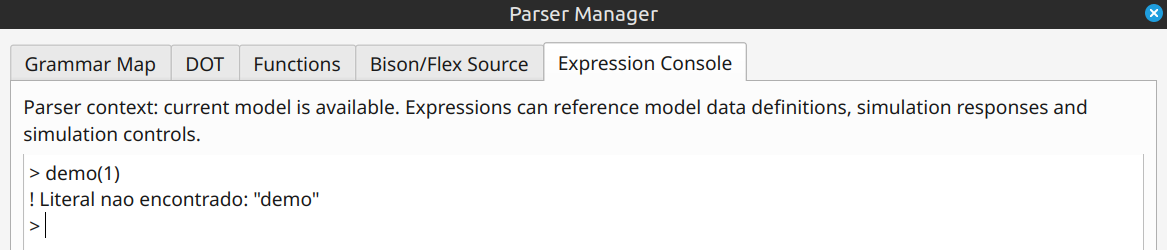
\includegraphics[width=\textwidth,height=0.44\textheight,keepaspectratio]{pre_demo.png}

        {\scriptsize Antes: \codeid{demo()} n\~ao reconhecida}

        \column{0.33\textwidth}
        \centering
        
\includegraphics[width=\textwidth,height=0.44\textheight,keepaspectratio]{demo_extension.png}

        {\scriptsize Extens\~ao declarada no modelo}

        \column{0.33\textwidth}
        \centering
        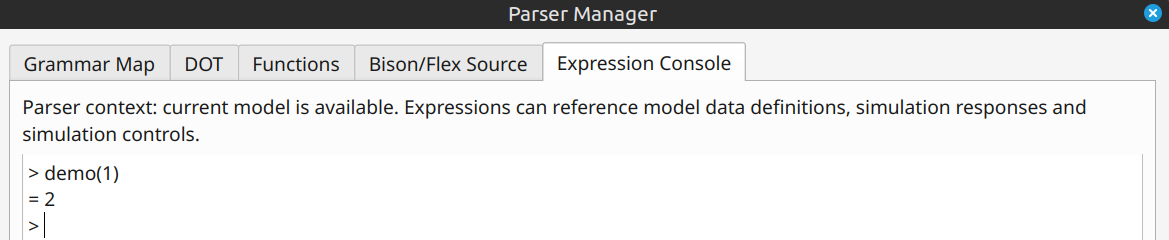
\includegraphics[width=\textwidth,height=0.44\textheight,keepaspectratio]{after_demo.png}

        {\scriptsize Depois: parser atualizado}
    \end{columns}

    \vspace{0.25cm}
    \begin{block}{Leitura do resultado}
        A fun\c{c}\~ao n\~ao existia na linguagem base; a extens\~ao declarou as mudan\c{c}as; o parser passou a reconhecer a express\~ao.
    \end{block}
\end{frame}

\begin{frame}{Resultados do Projeto}
    \begin{itemize}
        \item Contratos previstos passaram a formar um fluxo funcional.
        \item Plugins podem declarar altera\c{c}\~oes l\'exicas e sint\'aticas.
        \item O parser \'e regenerado sob demanda com Bison, Flex e C++.
        \item A biblioteca gerada \'e carregada em runtime por uma factory C.
        \item Falhas preservam o parser anterior e retornam diagn\'osticos.
    \end{itemize}

    \vspace{0.25cm}
    \begin{alertblock}{Mensagem final}
        A linguagem de express\~oes do GenESyS passa a acompanhar dinamicamente as extens\~oes carregadas no modelo.
    \end{alertblock}
\end{frame}

\begin{frame}{Encerramento}
    \centering
    {\Large Obrigado!}

    \vspace{0.6cm}
    \begin{block}{Tema}
        Mecanismo de atualiza\c{c}\~ao din\^amica do parser no GenESyS.
    \end{block}

    \vspace{0.25cm}
    {\small Perguntas?}
\end{frame}

\end{document}
